\chapter{Experiments and Results}
\label{chap:ExperimentsAndResults}

TODO: quick chapter overview

\begin{code}
$ python3 main.py unet train --val_pages 123 ...
\end{code}


\section{Architecture}
\label{sec:Architecture}


\section{Datasets}
\label{sec:Datasets}


\section{Semi-supervised Improvements}
\label{sec:SemisupervisedImprovements}

The main hypothesis this work is attempting to validate is that adding unlabelled data to the training process helps. We primarily want to improve model accuracy, but as we will see, this is not what our experiments suggest. They do, however, show improvements in other areas, such as training stability and reduced overfitting (section \ref{sec:UtilizingCvcMuscima}).

In the first experiment, we test how various labeled to unlabeled data ratios affect the training process. The experiment uses the MUSCIMA++ dataset [CITE]:

\begin{itemize}
    \item 10 pages act as the labeled set.
    \item 0, 5, 10 and 50 pages act as the unlabeled set.
    \item 10 pages act as the validation set.
    \item All of these pages come from the writer-independent train set of MUSCIMA++ and are chosen in a writer-independent manner (all the splits contain pages by different writers).
\end{itemize}

The learned task is notehead segmentation (both full and empty noteheads). Noteheads are an ideal symbol for this kind of measurement. Firstly, they are very abundant. Each page of the dataset contains many instances of them and they are evenly scattered over the whole page. If we were to instead detect more rare symbols (such as clefs or rests), it could skew the results, making it difficult to separate the effects we want to measure. Handwritten noteheads are also very diverse in style, making them more interesting to learn (compared to, say, stafflines).

All model hyperparameters are set to sensible deafults. The derivation of these values is desribed later in section \ref{sec:UnderstandingHyperparameters}. The model capacity, described by the \emph{inner features} parameter is set to 8, which is useful to know for comparison with the next experiment. The proposed dataset is rather small and so the training is very noisy (figure \ref{fig:ExplorationNoteheadsNoDropout}). To stabilize the trainig we set the dropout parameter to 50\% [CITE DROPOUT].

\begin{figure}[ht]
    \centering
    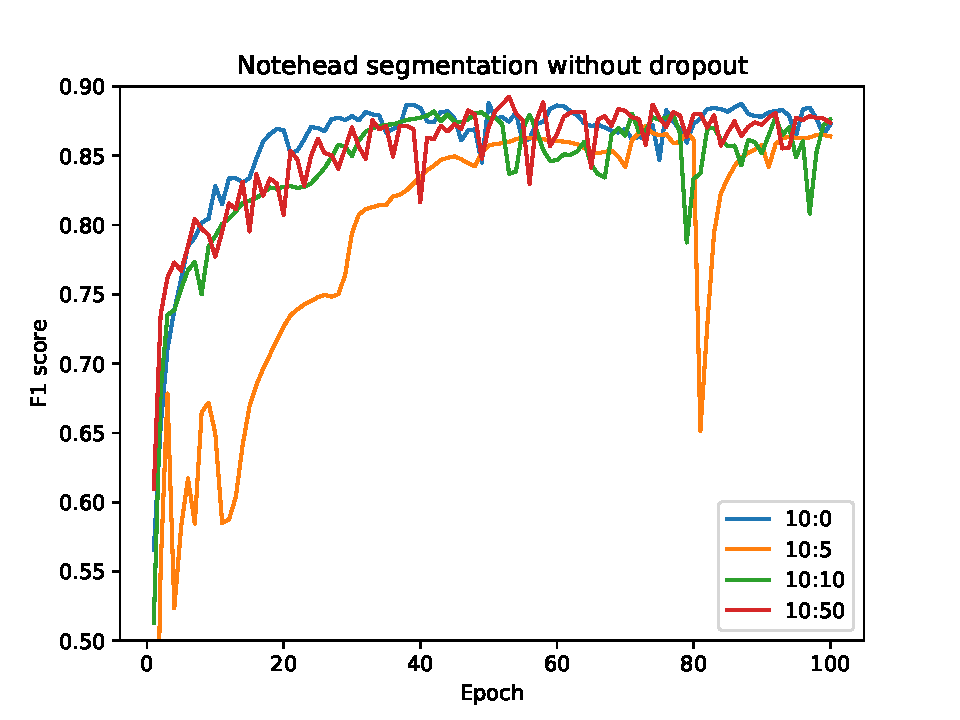
\includegraphics[width=140mm]{../../figures/01-exploration-noteheads/noteheads.pdf}
    \caption{Training on a small dataset without dropout is noisy, see the orange line at the beginning and the green line at the end.}
    \label{fig:ExplorationNoteheadsNoDropout}
\end{figure}

We expect that as we add more and more unlabeled data, the F1 score should reach higher and higher. Or at least not get worse. This is not what we see in the figure \ref{fig:ExplorationNoteheads}. The fully supervised model outperforms all the others by a clear margin.

Focusing only on the semi-supervised models, it seems that adding more unsupervised data maybe helps here, although the three lines end up on top of each other at the epoch 200. A better idea is to look at the figure \ref{fig:ExplorationNoteheadsEvaluation}. The chart contains evaluation results on the test set of six runs of each configuration. We can clearly see how the performance rises with more unsupervised data. Unfortunately it does not reach above the fully-supervised results. We unfortunately cannot push the amount of unlabeled data much higher, as it would break our training process (see section \ref{sec:BatchSize}) and it would likely also have diminishing returns. The actual numbers are summarized in table \ref{tab:ExplorationNoteheads}.

The reason for the drop in performance is actually caused by the fact, that the supervised model has to only learn one task -- segmentation. Whereas the semi-supervised one has to also learn the unsupervised reconstruction task. This claim is explored in the next section and is supported by the fact that the performance drop disappears when we increase model capacity.

\begin{figure}[p]
    \centering
    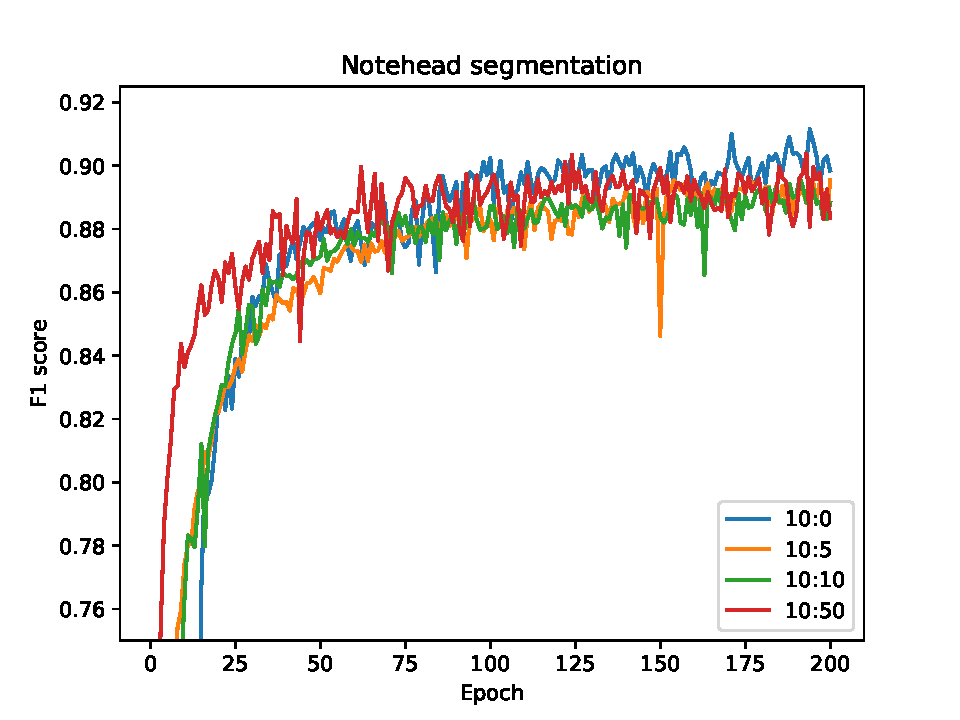
\includegraphics[width=140mm]{../../figures/01-exploration-noteheads/noteheads-dropout.pdf}
    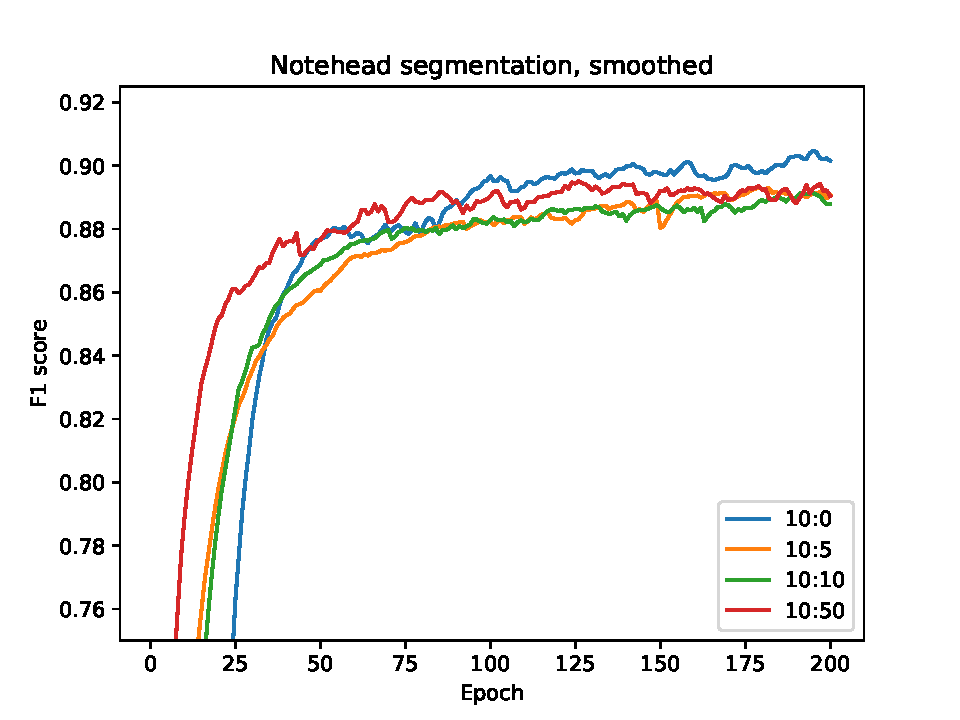
\includegraphics[width=140mm]{../../figures/01-exploration-noteheads/noteheads-dropout-smooth.pdf}
    \caption{Lorem ipsum dolor.}
    \label{fig:ExplorationNoteheads}
\end{figure}

\begin{figure}[ht]
    \centering
    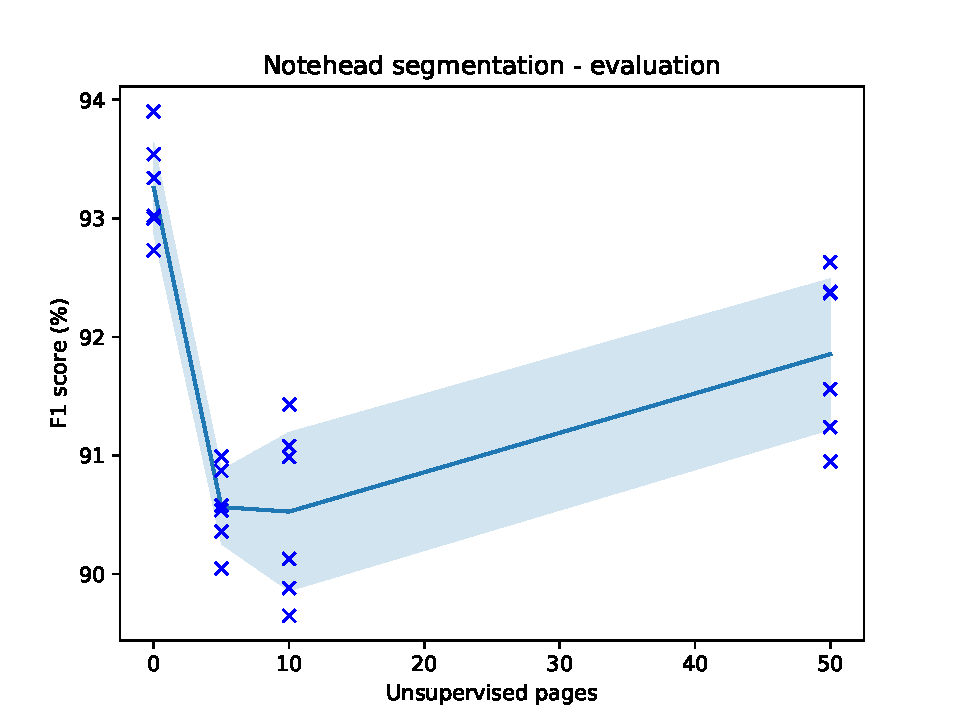
\includegraphics[width=140mm]{../../figures/01-exploration-noteheads/noteheads-evaluation.pdf}
    \caption{Lorem ipsum dolor.}
    \label{fig:ExplorationNoteheadsEvaluation}
\end{figure}

\begin{table}[b!]
    \centering
    \begin{tabular}{l@{\hspace{1.5cm}}D{.}{,}{3.2}D{.}{,}{1.2}D{.}{,}{2.3}}
        \toprule
        & \mc{} & \mc{\textbf{Směrod.}} & \mc{} \\
        \pulrad{\textbf{Efekt}} & \mc{\pulrad{\textbf{Odhad}}} & \mc{\textbf{chyba}$^a$} &
        \mc{\pulrad{\textbf{P-hodnota}}} \\
        \midrule
        Abs. člen     & -10.01 & 1.01 & \mc{---} \\
        Pohlaví (muž) & 9.89   & 5.98 & 0.098 \\
        Výška (cm)    & 0.78   & 0.12 & <0.001 \\
        \bottomrule
    \end{tabular}
    \caption{Lorem ipsum dolor.}
    \label{tab:ExplorationNoteheads}
\end{table}

TODO: show visualization images / qualitative comparison between runs?


\section{Utilizing CVC-MUSCIMA}
\label{sec:UtilizingCvcMuscima}

This experiment attempts to address issues of the previous experiment:

\begin{itemize}
    \item fixed model capacity
    \item small dataset
\end{itemize}

In the chapter \ref{chap:CurrentStateOfOMR} we described the two major datasets for handwritten music recognition: CVC-MUSCIMA [CITE] and MUSCIMA++ [CITE]. The dataset MUSCIMA++ is a highly annotated subset of CVC-MUSCIMA. We can view both datasets together as a single semi-supervised dataset, being 12\% labeled and 88\% unlabeled. To the best of our knowledge, nobody has yet tried to utilize both datasets simulatenously for semantic segmentation.

Hajič jr. and Dorfer [CITE 1, 2] have used the U-Net architecture [CITE] for segmentation and they trained it on the MUSCIMA++ dataset. Their results are very impressive. Being able to further build on their work and improving the model by utilizing unlabeled data from CVC-MUSCIMA would be very helpful for the field of OMR. This experiment attempts to do just that.

We take the whole CVC-MUSCIMA dataset, separate writers from the MUSCIMA++ independent test set, separate 20 pages for validation set and remove other pages from these validation writers. The pages that remain are produced by writers not present in both the test set and the validation set. These remaining pages are partially contained in the MUSCIMA++ dataset (99 pages) and all the other pages are used as unlabeled data (551 pages). Therefore we train on 650 out of 1000 pages of the CVC-MUSCIMA dataset.

Since the dataset is now much larger than in the previous experiment (section \ref{sec:SemisupervisedImprovements}), we no longer need the dropout. In fact, the training is even more stable and individual runs are clearly separated.

This experiment attempts to compare fully-supervised and semi-supervised models, regardless of their capacity. We therefore train various model capacities (the \emph{inner features} model parameter) and then compare the best ones for each setting.

Another difference to the previous experiment is that the ratio of labeled to unlabeled data is fixed and given by dataset sizes. The ratio of 99 to 551 pages corresponds best with the ratio 10:50.

\begin{figure}[p]
    \centering
    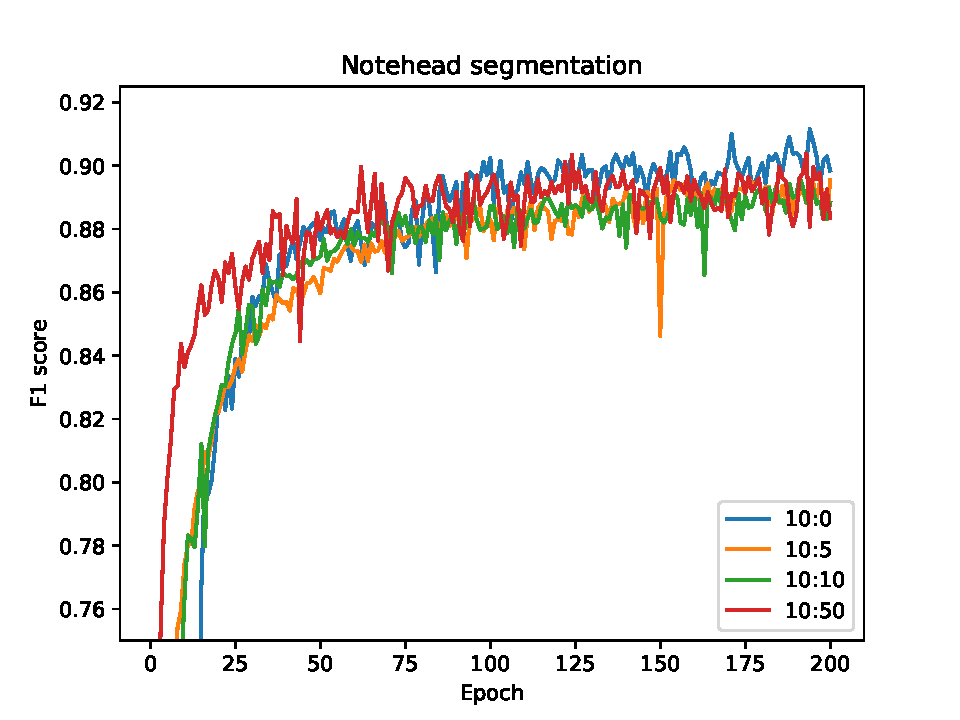
\includegraphics[width=140mm]{../../figures/01-exploration-noteheads/noteheads-dropout.pdf}
    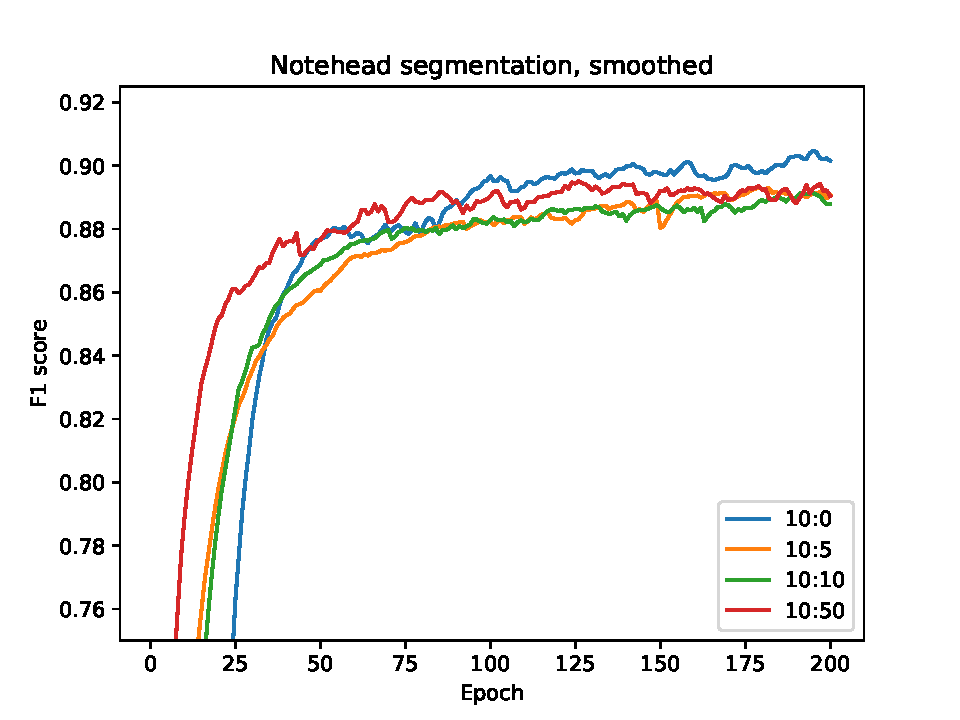
\includegraphics[width=140mm]{../../figures/01-exploration-noteheads/noteheads-dropout-smooth.pdf}
    \caption{Lorem ipsum dolor. TODO: the two improvements charts}
    \label{fig:CvcImprovements}
\end{figure}

The validation dataset F1 score over the course of training can be seen in figure \ref{fig:CvcImprovements}. In these charts we can see:

\begin{itemize}
    \item Models with 1 and 2 \emph{inner features} are clearly underfitting in the supervised mode (compared to other models). When we add the unlabeled data, their perfomance drops significantly, but the training curve gets much smoother.
    \item Models with 4 and 8 \emph{inner features} worsen much less and also get smoother (especially 4 becomes much more stable).
    \item Model 16 no longer worsens, it is able to learn both tasks.
\end{itemize}

TODO: try training the 32ft semi-supervised model, it could maybe get over the bar...

Conclusions can be drawn from these observations:

\begin{itemize}
    \item The reconstruction and segmentation tasks clearly compete for model capacity. The performance drop of adding unlabeled data decreases, as the model capacity increases.
    \item The addition of unlabeled data can be used as a regularization technique. This is evident from the fact that training curves get much smoother as we add unlabeled data. A~regularization effect is also described in the corresponding literature [CITE SSL overview].
    \item All models come close to the 96\% line, but never cross it. While the semi-supervised models get as good as the fully-supervised, they never get better. It seems the reconstruction task is not learning any useful representations. [TODO: expand on this further and show reconstruction visualizations - they learn simple shapes, not abstract objects]
\end{itemize}

% TODO: evaluate best models of SUP and SEMISUP, maybe they differ in test score? Probbably not.


\section{Knowledge Transfer}
\label{sec:KnowledgeTransfer}

TODO: knowledge transfer experiment

\section{Understanding Hyperparameters}
\label{sec:UnderstandingHyperparameters}


\subsection{Batch Size}
\label{sec:BatchSize}

In the deep learning field, it is known that having a small batch size makes the training fast and noisy, whereas a large batch size makes it more stable at the cost of being slower [CITE DL BOOK]. Since our model is fully cconvolutional and we train it on image tiles of fixed size, we can consider the size of these tiles to be a parameter similar to batch size. It also regulates the amount of data used for gradient estimation. If the tiles are large enough, we can get away with batch size of 1 (this is what the original U-Net article does [CITE]).

Using such a small batch size is, however, not possible in our case. Our training process expects batches containing both labeled and unlabeled data. Batch size determines the total number of these two kinds of data items in the single composite batch. The ratio of these two item types within the composite batch is dictated by the ratio within the whole dataset. So if our dataset has, for example, 1:5 labeled to unlabeled data, the batch size has to be at-least 6. Otherwise we will start getting batches that contain only unlabeled data. This rule isn't as strict, since the model would probably learn both tasks even if half of all batches were missing labeled data, however if the imbalance becomes too severe, the training fails.

TODO: figure with the failing training (bs=2,ratio=1:10)

An example of such a failing training can be seen in figure TODO???. The model learns to perform reconstruction even for the segmentation task. This is understandable, since the two tasks are differentiated only at the last layer (1x1 sigmoid convolution). If all second-to-last layer activations contain image reconstruction data, then any 1x1 convolution combination of them will do as well.

Since all of our experiments have training data ratios between 1:0 and 1:10, we chose to set the batch size parameter to 10.


\subsection{Dropout}
\label{sec:Dropout}

We introduced dropout [CITE] when training on small datasets (section \ref{sec:SemisupervisedImprovements}). The training was so noisy, that it was difficult to infer any measurable differences between runs. Therefore we used dropout as a mean to stabilize the training. The model performace also sligtly increased in this setting.

When we train on larger datasets, the training is no longer unstable and dropout is not needed (section \ref{sec:UtilizingCvcMuscima}). In fact, it causes the training process to converge much slower (2x or more) and it does not perform any better.

Both the original U-Net article [CITE] and the article by Hajič jr. et al. [CITE] use the U-Net architecture without any dropout. In fact, an article by Thompson et al. [CITE] argues, that using traditional dropout on convolutional layers may not be ideal. This agrees with our findings, that dropout helps only in very specific circumstances.

From this we conclude that dropout should be disabled by default.


\subsection{Skip Connections}

\subsection{Unsupervised Loss Weight}

\subsection{Activation Function}
